\documentclass{article}

\usepackage[french]{babel}
\usepackage[utf8]{inputenc}
\usepackage[T1]{fontenc}
\usepackage{graphicx}
\usepackage{algorithm}
\usepackage{algorithmic}

%%%%%%%%%%%%%%%% Lengths %%%%%%%%%%%%%%%%
\setlength{\textwidth}{15.5cm}
\setlength{\evensidemargin}{0.5cm}
\setlength{\oddsidemargin}{0.5cm}

%%%%%%%%%%%%%%%% Variables %%%%%%%%%%%%%%%%
\def\project{5}
\def\title{Interpolation de surface et méthodes d'integration}
\def\group{3}
\def\team{5}
\def\manager{Mohamed Faycal Boullit}
\def\secretary{Lucas Guédon}
\def\others{Imad Boudroua, Enzo Mezzasalma, Simon Triscos}

\begin{document}

%%%%%%%%%%%%%%%% Header %%%%%%%%%%%%%%%%
\noindent\begin{minipage}{0.98\textwidth}
  \vskip 0mm
  \noindent
  { \begin{tabular}{p{6.5cm}}
      {\bfseries \sffamily
        Project \project} \\ 
      {\itshape \title}
    \end{tabular}}
  \hfill 
  \fbox{\begin{tabular}{p{8cm}}
      {~\hfill \bfseries \sffamily Group \group\ - Team \team
        \hfill~} \\[2mm] 
      Responsable : \manager \\
      Secrétaire : \secretary \\
      Développeurs : \others
    \end{tabular}}
  \vskip 4mm ~

  ~~~\parbox{0.95\textwidth}{\small \textit{Résumé :} \sffamily Le but de ce projet est d'utiliser les méthodes d'interpolation et d'intégration de fonctions afin de modéliser le flux d'aire autour d'une aile d'avion.}
  \vskip 1mm ~
\end{minipage}

%%%%%%%%%%%%%%%% Main part %%%%%%%%%%%%%%%%

\section{Interpolation}

L'objectif de cette partie est d'expliquer l'implémentation de splines cubiques utilisé pour obtenir une fonction à partir de points de la coupe d'une aile d'avion.

\subsection{Implémentation}

L'algorithme de la spline cubique est donné dans le chapitre 3 de Numerical Recipes. Il a été adapté pour fonctionner sur python. Les vecteurs ont été remplacés par des tableaux de numpy. Afin de pouvoir utiliser une seule fonction pour calculer une spline, une fonction $spline\_fun$ a été créée. Celle-ci calcul la dérivée seconde de chaque point en entrée et retourne la spline sous la forme d'une fonction que l'on peut appliquer à un paramètre x pour obtenir la valeur de la spline en x en utilisant les dérivées secondes trouvées précédemment.

\subsection{Tests}

La méthode a été testée sur la coupe d'aile de k1. Afin de visualiser le résultat, nous avons affiché sur le même graphique la fonction obtenue grâce à la spline cubique et les points originaux de l'aile.

\begin{figure}[!htb]
    \centering
    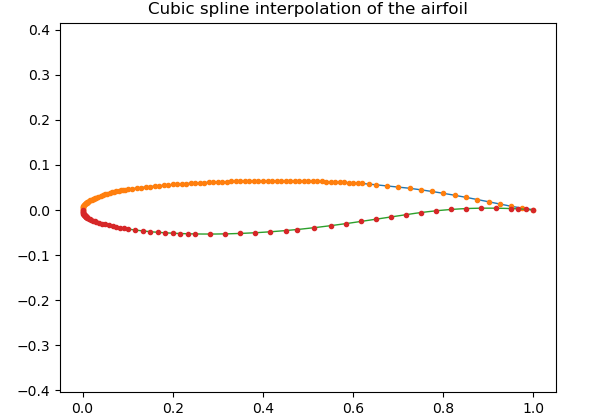
\includegraphics[width=0.57\textwidth]{airfoil.png}
    \caption{Interpolation du profil d'aile de l'avion grâce à une spline cubique}
    \label{airfoil_profil}
\end{figure}


\section{Intégration de la fonction}

Cette section a pour but de montrer les différentes méthodes d'intégrations qui ont été implémentées et de montrer leurs différences en terme d'efficacité.

\subsection{Implémentations}

Nous avons tout d'abord choisit d'implémenter une technique simple permetant de calculer l'intégrale d'une fonction. Nous avons donc implémenter la méthode des rectangles à gauche.
Pour ce faire, nous avons créé une fonction qui à partir de la fonction à intégrer, de l'intervalle sur lequel intégrer et de la précision $epsilon$ va calculer l'intégrale. La méthode fonctionne par itérations progressives. À chaque étape, le pas est divisé par deux et la valeur calculée à l'étape précédente est réutilisée pour minimiser le nombre d'appels à la fonction originale.

Nous avons également implémenté la méthode des rectangles du point milieu pour avoir une implémentation plus efficace. Avec cette méthode est d'ordre $1$ et le pas est divisé par 3 à chaque étape.

\subsection{Comparaison des méthodes}

Afin de comparer l'efficacité des méthodes implémentées, nous avons tracé en Figure \ref{erreur_abs} l'erreur absolue de la valeur calculée en fonction du nombre d'appels à la fonction. Nous avons choisi la fonction $f(x) = x^2 + 2$ sur l'intervalle $[0, 1]$ pour pouvoir comparer le résultat des méthodes avec une intégrale réelle connue. Ainsi, on peut examiner la vitesse de convergence des méthodes pour minimiser le nombre d'appels à $f$.

On peut observer que la méthode des rectangles à gauche nécessite plus de 100 fois plus d'appels à $f$ que la méthode du point milieu pour calculer une intégrale avec une erreur absolue de $10^{-4}$.

\begin{figure}[!htb]
    \centering
    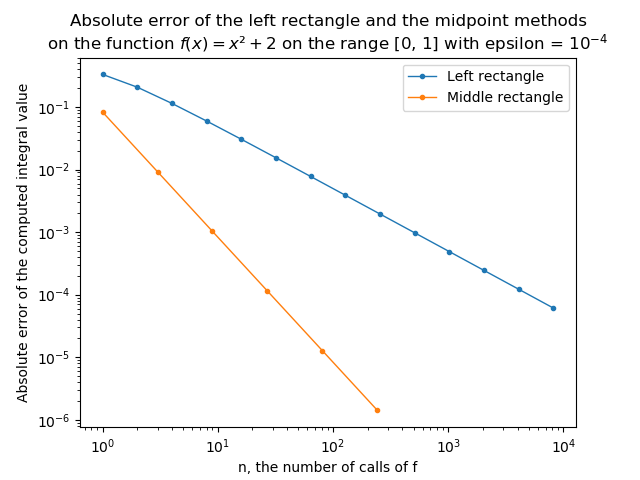
\includegraphics[width=0.66\textwidth]{error_integration_plot.png}
    \caption{Erreur absolue de chaque méthode d'intégration en fonction du nombre d'appels à $f$}
    \label{erreur_abs}
\end{figure}

\section{Modélisation du flux de l'air autour de l'aile}

Cette partie a pour objectif de montrer l'application des méthodes expliquées dans les sections précédentes pour modéliser le flux d'air autour d'une aile d'avion et produire une carte de la pression de l'air.

\subsection{Modélisation du flux laminaire}

Afin de modéliser le flux d'air, on considère qu'il s'agit d'un écoulement laminaire. C'est-à-dire que l'air peut être divisé en couches. Les couches proches de l'aile épousent la forme de l'aile et plus on s'éloigne, plus les couches deviennent droites comme montré sur la figure 3. Les couches sont modélisées par une fonction paramétrée par $\lambda \in [0, 1]$.

\begin{figure}[!htb]
    \centering
    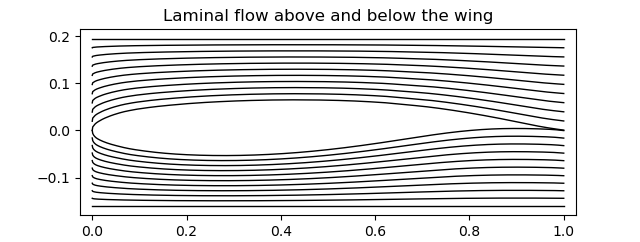
\includegraphics[width=1.04\textwidth]{laminar_flow.png}
    \caption{Visualisation de l'écoulement laminaire d'air autour de l'aile}
    \label{laminar_flow}
\end{figure}

\subsection{Modélisation de la pression}

Afin d'obtenir une carte de la pression, il est nécessaire de pouvoir calculer la pression à un point donné.
Pour ce faire, il faut calculer le facteur $\lambda$ qui correspond à la couche d'aire à ce point, cette couche qui est définie par la fonction $f_{\lambda}$ qui dépend principalement de la courbe définissant le coté de l'aile:
\begin{equation}
    f_{\lambda} = (1-\lambda)f(x) + \lambda \times 3hmax
\end{equation}
avec $hmax$ correspondant au maximum atteint par la courbe $f(x)$ sur l'intervalle $[0;1]$.
\\
La pression en question est définit alors par l'équation \ref{Pressure_eq} avec $V$ la vitesse en ce point :
\begin{equation}
    \label{Pressure_eq}
    P = P_s + \frac{1}{2} \times \rho \times V^2
\end{equation}
Comme le flux est laminaire, on peut considérer que l'air met un temps constant à traverser la coupe quel que soit la couche concernée. La vitesse est donc proportionnelle à la longueur de la couche.

\newpage
\subsection{Implémentation}
La proportionnalité entre la vitesse $V$ et la longeur $L$ et l'équation de la pression \ref{Pressure_eq} implique que la pression est proportionnelle à $L^2$, donc on a : $P \sim L^2$.\\
La longeur de la courbe est définit comme de suite: 
\begin{equation}
    L([0;T]) = \int_0^{T}\sqrt{1+f'(x)^2}dx
\end{equation}
la méthode utilisée pour le calcul de cette intégrale est la méthode du point milieu puisqu'elle est plus performante que la méthode des rectangles au niveau du temps de calcul, la precision du calcul de l'intégrale est de $10^{-2}$ puisqu'une précision plus petite prend plus de temps.

\subsection{Résultats}

La pression calculée autour de l'aile k1 est disponible en figure \ref{pressure_map}.
\begin{figure}[!htb]
    \centering
    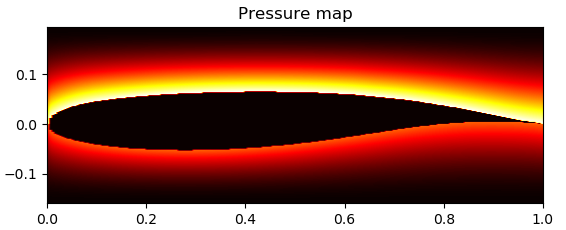
\includegraphics[width=1.04\textwidth]{pressure_map.png}
    \caption{Pression de l'air autour de l'aile}
    \label{pressure_map}
\end{figure}
\\
Le résultat obtenues illustre bien la pression de l'air élevée autour de l'aile, et une pression moins importante loin de ses cotés, ce qui vérifie bien notre proportionnalité utilisée.
La complexité résultante et qui apparait lors de l'éxecution de programme est dûe au fait que le programme calcul une intégrale à chaque position prise par la fonction $airflow\_pressure\_map$ alors que le nombre de position est de l'ordre de $10^{4}$, ce qui explique bien la durée prise lors du calcul de la pression autour de l'aile surtout en choisissant $espsilon$ très petit, pour cela on se suffit de $\varepsilon = 10^{-2}$, pour une optimisation au niveau du temps de calcul et un affichage correcte comme celui de la figure \ref{pressure_map}.
\begin{figure}[!ht]
    \centering
    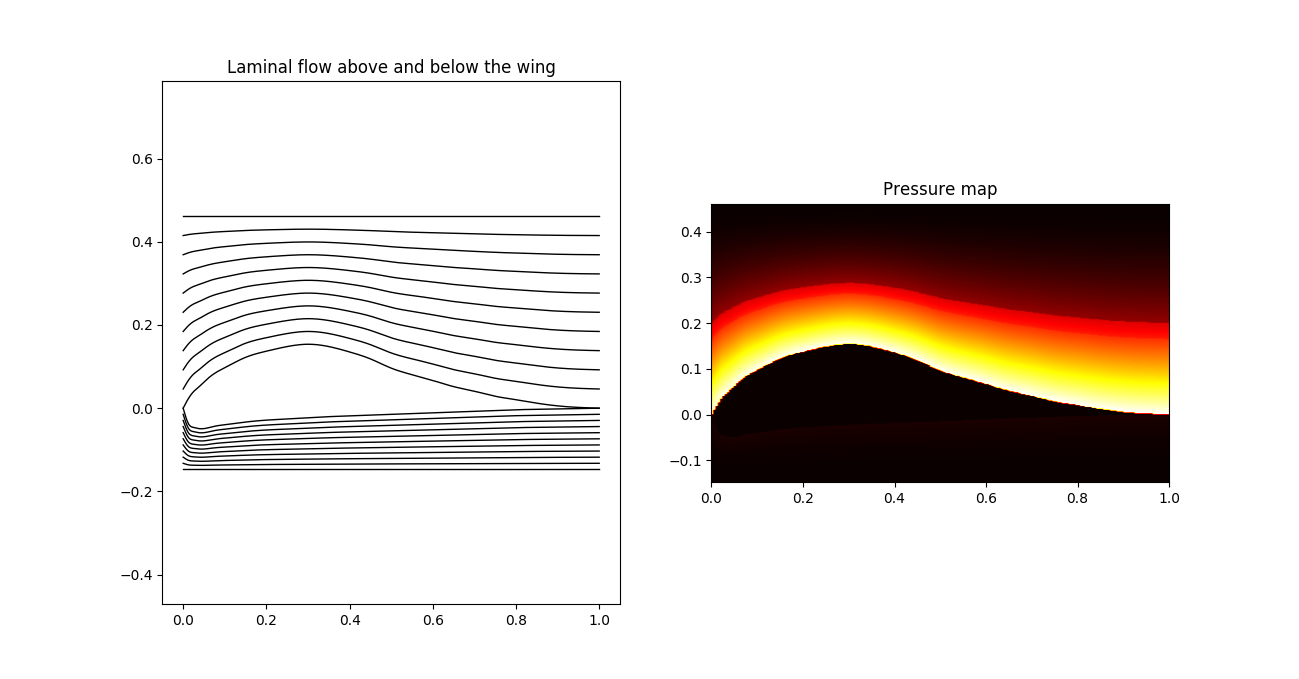
\includegraphics[width=1.04\textwidth]{pressure_map_L1003.png}
    \caption{Deuxième exemple du flux et de la pression de l'air autour de l'aile}
    \label{pressure_map_L1003}
\end{figure}
\\
\\
\\
\\
\\
\\
Ce deuxième exemple présenté dans la figure \ref{pressure_map_L1003}, représente le flux et la pression de l'aire autour de l'aile L1003, cette exemple illustre bien la proportionnalité entre la pression et la longeur des couches, comme on peut remarque au niveau inférieur de l'aile ou les couches sont peu courbées, la pression est moin importante, alors qu'au niveau supérieur de l'aile ou la courbure est remarquable on remarque la pression importante appliquée à ce niveau. Cette illustration de la pression aux différents niveaux de l'aile peut également aider les spécialistes des ailes dans leur construction, afin d'éviter une surpression qui peut endommager l'aile et analyser sa capacité de maintenir l'avion en air.

\section{Conclusion}
Les méthodes d'intégration implémentées ont été de différentes complexité, la méthode du point milieu était la plus performante et la plus optimisée, c'est celle utilisée pour calculer les intégrales afin d'obtenir la pression après avoir affiner le profil aérodynamique en une courbe suffisament lisse.

\end{document}